\documentclass[]{article}
\usepackage{ifxetex,ifluatex}
\ifnum 0\ifxetex 1\fi\ifluatex 1\fi=0 % if pdftex
\usepackage[T1]{fontenc}
\usepackage[utf8]{inputenc}
%\setcounter{secnumdepth}{0}
\usepackage[table,xcdraw]{xcolor}
\usepackage[margin=1.5in]{geometry}
\usepackage[tableposition=top]{caption}
\usepackage{tabularx}
\usepackage{hyperref}
\usepackage{graphicx}
\hypersetup{
colorlinks=true,
linkcolor=blue,
filecolor=magenta,
urlcolor=cyan,
}



\title{\textbf{Patients Transit Visualizer}\\Specyfikacja implementacyjna projektu zespołowego}
\author{\small{AiSD GR2}\\Martyna Jakubowska, Hubert Nakielski, Artur Prasuła}
\date{Grudzień 2020}


\begin{document}
    \maketitle
    \newpage
    
    \section{Informacje Ogólne} % Artur
    Program można uruchomić za pomocą naciśnięcia myszką na ikonę programu.
    Dlatego też, program nie przyjmuje żadnych parametrów uruchomieniowych.
    Okno programu po włączeniu będzie mieć rozmiar 800x600 pikseli.
    Dzięki temu, program zmieści się niemalże na każdym sprzęcie.
    Dodatkowo rozmiar okna, będzie mógł zostać zmieniony ręcznie przez użytkownika.
    Program pojawi się na ekranie tak, aby środek okna programu był środkiem monitora użytkownika.
    Wyłączenie programu będzie możliwe za pomocą przycisku w prawym górnym rogu programu.
    
    
    \section{Diagram klas} % Artur
        \begin{figure}[!h]
            \centering
            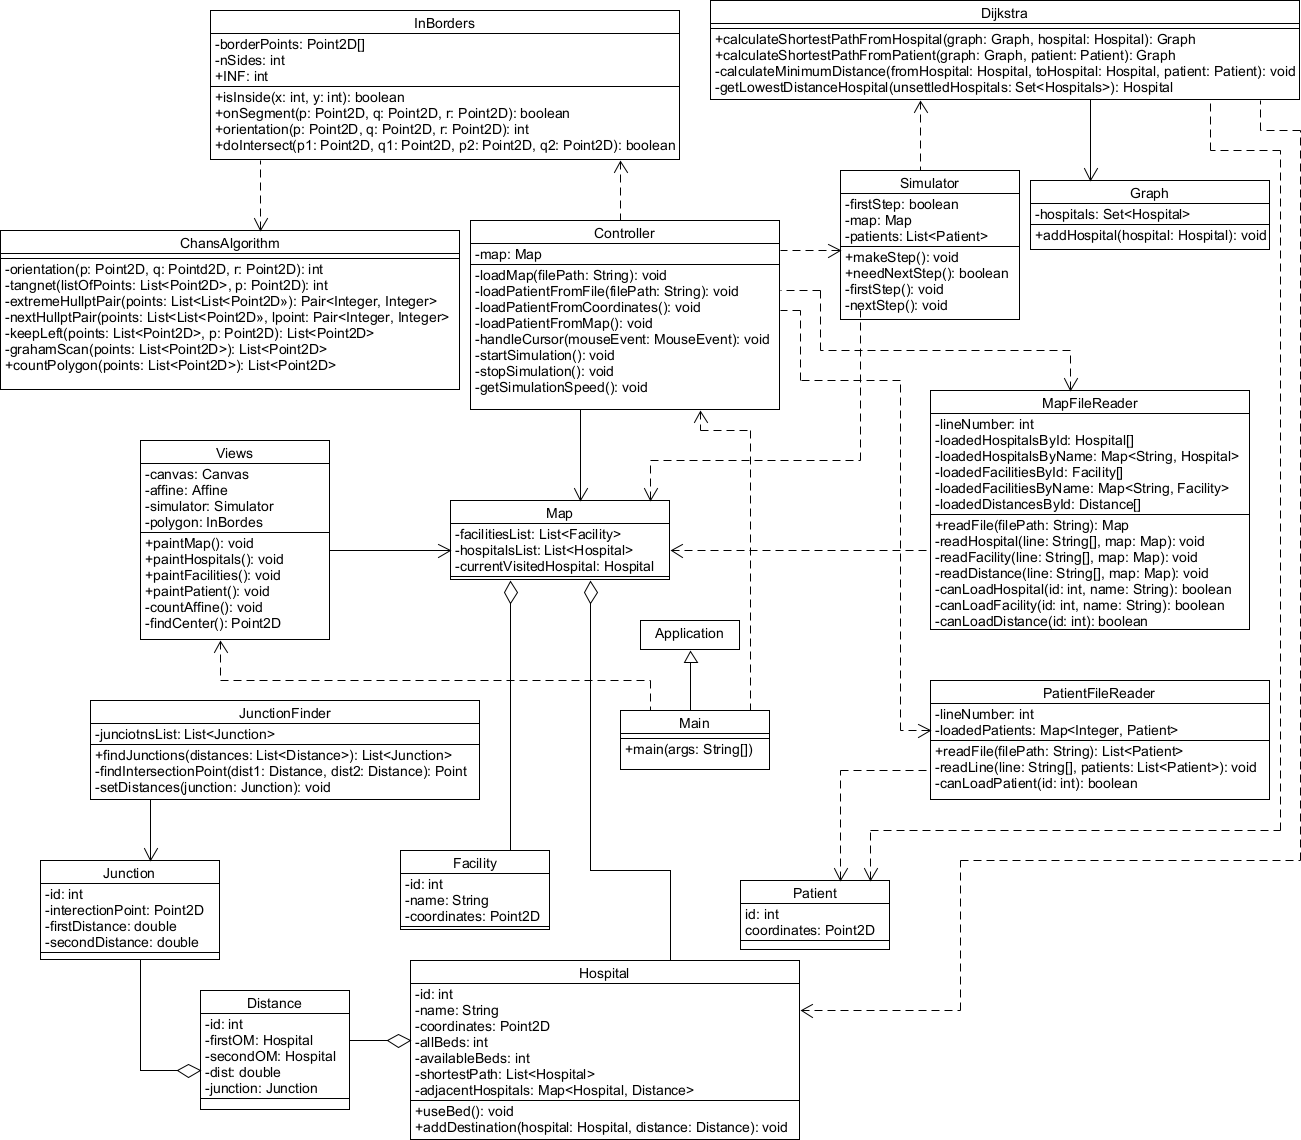
\includegraphics[width=\textwidth]{diagram_klas.png}
            \caption{Diagram klas}
            \label{fig:Diagram klas}
        \end{figure}
    
    
    \section{Opis pakietów}
        \subsection{ptv}
        Pakiet ten zajmuje się obsługą całego programu. Przechowywane są w nim wszystkie występujące pakiety.
        \subsection{ptv.module}
        Jest to pakiet przechowujący całą logikę programu. W tym pakiecie znajdują się obiekty służące do 
        wykonywania operacji związanych z funkcjonalnością programu.
        \subsection{ptv.module.path} % Hubert
        Pakiet \textbf{ptv.module.path} odpowiada za rozwiązanie problemu najkrótszej drogi. 
        Znajduje najkrótszą drogę do szpitala (OM) zarówno z dowolnego pola na mapie (zawartego w granicach), 
        jak i z istniejącego już OM. 
                    
    \subsubsection{Graph}
            Klasa ta reprezentuje graf z węzłami będącymi OM.
                
                \paragraph{Pola}
                    \begin{itemize}
                        \item \textbf{private Set<Hospital> hospitals} - przechowuje zbiór OM
                    \end{itemize}
            
                \paragraph{Metody}
                    \begin{itemize}
                        \item \textbf{public void addHospital(Hospital hospitalA)} - Metoda dodaje OM do zbioru 
                    \end{itemize}
                
                
            \subsubsection{Dijkstra} 
            Ta klasa implementuje algorytm Dijkstry, służy ona do obliczenia najkrótszej możliwej drogi.
                
                \paragraph{Pola}
                     brak
                    
                \paragraph{Metody}
                    \begin{itemize}
                        \item \textbf{public Graph calculateShortestPathFromHospital(Graph graph, Hospital hospital)} - 
                            Metoda, używając \textit{calculateMinimumDistance} i \textit{getLowestDistanceHospital}, 
                            znajduje najkrótsze drogi pomiędzy wszystkimi szpitalami. Uwzględnia ona zarówno drogi wczytane z 
                            pliku, jak te prowadzące przez skrzyżowania.
                        \item \textbf{public Graph calculateShortestPathFromPatient(Graph graph, Patient patient)} - 
                            Metoda ta znajduje drogę i szpital do którego Karetka Pogotowia jest w stanie przewieźć pacjenta jak najszybciej.
                        \item \textbf{private void calculateMinimumDistance(Hospital fromHospital, Hospital toHospital, Integer edgeWeigh)} - 
                            Metoda ta znajduje najkrótszą drogę pomiędzy dwoma szptalami. Bierze pod uwagę drogi 
                            wczytane z pliku wejściowego oraz drogi powstałe z ustalenia skrzyżowań.
                        \item \textbf{private Hospital getLowestDistanceHospital(Set<Hospital> unsettledHospitals)} - 
                            Zwraca OM, do którego w danej chwili prowadzi najkrótsza droga. Bierze pod uwagę tylko te OM, 
                            których najkrótsze drogi nie zostały jeszcze ustalone.
                    \end{itemize}
                
        
        \subsection{ptv.module.data} % Hubert
        Pakiet \textbf{ptv.module.data} przechowuje klasy odpowiedzialne za definicję obiektów niezbędnych do działania programu.
        
            \subsubsection{JunctionFinder}
                    Klasa ta oblicza i znajduje skrzyżowania dróg, które zostały wprowadzone z pliku wejściowego.
                \paragraph{Pola}
                    \begin{itemize}
                        \item \textbf{private List<Junction> junctionsList} - tu przechowywana jest lista skrzyżowań
                    \end{itemize}
            
                \paragraph{Metody}
                    \begin{itemize}
                        \item \textbf{public List<Junction> findJunctions(List<Distance>)} -
                            Metoda znajduje wszystkie skrzyżowania i zwraca ich listę. Używa metod \textit{fintIntersectionPoint} i 
                            \textit{setDistances}.
                        \item \textbf{private Point findIntersectionPoint(Distance dist1, Distance dist2)} - 
                            Metoda ta znajduje punkt przecięcia się dwóch dróg i go zwraca.
                        \item \textbf{private void setDistances(Junction junction)} - 
                            Metoda ta ustala odległości dróg: od pierwszego OM do skrzyżowania i od skrzyżowania do drugiego OM.
                    \end{itemize}
                    
            \subsubsection{Junction}
                Przechowuje definicję obiektu drogi ze skrzyżowaniem.
                    
                \paragraph{Pola}
                    \begin{itemize}
                        \item \textbf{private int id} - przechowuje id skrzyżowania
                        \item \textbf{private Point2D intersectionPoint} - przechowuje współrzędne skrzyżowania
                        \item \textbf{private double firstDistance} - przechowuje długość pierwszej drogi tj. od pierwszego OM do skrzyżowania
                        \item \textbf{private double secondDistance} - przechowuje długość drugiej drogi tj. od skrzyżowania do drugiego OM
                    \end{itemize}
            
                \paragraph{Metody}
                    Metody dostępowe
              
                    
            \subsubsection{Hospital}
                    Przechowuje definicję obiektu Ośrodka Medycznego (OM).
                \paragraph{Pola}
                    \begin{itemize}
                        \item \textbf{private int id} - przechowuje id OM
                        \item \textbf{private String name} - przechowuje nazwę OM
                        \item \textbf{private Point2D coordinates} - przechowuje współrzędne OM
                        \item \textbf{private int allBeds} - przechowuje liczbę wszystkich łóżek
                        \item \textbf{private int avaliableBeds} - przechowuje liczbę dostępnych łóżek
                        \item \textbf{private LinkedList<Hospital> shortestPath} - przechowuje listę najkrótszych dróg do innych OM
                        \item \textbf{private Map<Hospital, Distance> adjacentHospitals} - przechowuje drogi do innych OM
                    \end{itemize}
            
                \paragraph{Metody}
                    \begin{itemize}
                        \item \textbf{public void useBed()} - 
                            Metoda ta odejmuje 1 od atrybutu \textit{avaliableBeds}, gdy zostawiamy pacjenta w OM.
                        \item \textbf{public void addDestination(Hospital destination, Distance distance)} - 
                            Metoda ta dodaje połączenie między tym OM, a innym OM.
                    \end{itemize}
                    
            \subsubsection{Facility}
                    Przechowuje definicję obiektu pewnego rodzaju budowli, np. Pomnik czy Muzeum
                \paragraph{Pola}
                    \begin{itemize}
                        \item \textbf{private int id} - przechowuje id obiektu
                        \item \textbf{private String name} - przechowuje nazwę obiektu
                        \item \textbf{private Point2D coordinates} - przechowuje współrzędne obiektu
                    \end{itemize}
            
                \paragraph{Metody}
                    Metody dostępowe
                    
            \subsubsection{Distance}
                    Przechowuje definicję obiektu drogi z jednego OM do drugiego OM.
                \paragraph{Pola}
                    \begin{itemize}
                        \item \textbf{private int id} - przechowuje id drogi
                        \item \textbf{private Hospital firstOM} - przechowuje OM, z którego prowadzi droga
                        \item \textbf{private Hospital second OM} - przechowuje OM, do którego prowadzi droga
                        \item \textbf{private double dist} - przechowuje bezjednostkową odległość drogi 
                        \item \textbf{private Junction junction} - jeśli występuje skrzyżowanie to przechowuje je
                    \end{itemize}
            
                \paragraph{Metody}
                    Metody dostępowe
                    
            \subsubsection{Patient}
                    Przechowuje definicję obiektu pacjenta
                \paragraph{Pola}
                    \begin{itemize}
                        \item \textbf{private int id} - przechowuje id pacjenta
                        \item \textbf{private Point2D coordinates} - przechowuje współrzędne pacjenta
                    \end{itemize}
            
                \paragraph{Metody}
                    Metody dostępowe
                    
            \subsubsection{Map}
                    Przechowuje listy wszystkich obiektów i OM dostarczonych w pliku wejściowym.
                \paragraph{Pola}
                    \begin{itemize}
                        \item \textbf{private List<Facility> facilitiesList} - przechowuje listę obiektów w programie, dostarczonych w pliku wejściowym 
                        \item \textbf{private List<Hospital> hospitalsList} - przechowuje listę OM w programie, dostarczonych w pliku wejściowym
                        \item \textbf{private Hospital currentVisitedHospital} - przechowuje OM, w którym aktualnie przebywa pacjent
                        \item \textbf{private List<Piont2D> polygon} - przechowuje OM oraz obiekty, które wyznaczają granice
                    \end{itemize}
            
                \paragraph{Metody}
                    Metody dostępowe
        
        \subsubsection{ChansAlgorithm}
                Klasa \textbf{ChansAlgorithm} implementuje algorytm Chana, służący do wyznaczania punktów granicznych
                \paragraph{Pola}
                    brak
                \paragraph{Metody}
                    \begin{itemize}
                        \item \textbf{private int orientation(Point2D p, Point2D q, Point2D r)} - metoda znajduje orientację 3 punktów, zwraca 0 -> p, q i r są współliniowe,1 -> Zgodnie z ruchem wskazówek zegara,2 -> Przeciwnie do ruchu wskazówek zegar
                        \item\textbf{ private int compare(Point2D p0, Point2D vp1, Point2D vp2)} - metoda służąca do porównywania punktów
                        \item \textbf{private int tangnet(List<Point2D> listOfPoints, Point2D p)} - zwraca index punktu do którego poprowadzona jest styczna z punktu p
                        \item \textbf{private Pair<Integer, Integer> extremeHullptPair(List<List>Point2D>{}> points)} - metoda zwracająca parę liczb całkowitych reprezentujących granicę i punkt krańcowy w tej granicy
                        \item \textbf{private Pair<Integer, Integer> nextHullptPair(List<List<Point2D>{}> points, Pair<Integer, Integer> lpoint)} - zwraca parę liczb całkowitych reprezentujących granicę i punkt na tej granicy, do którego zostanie połączony punkt
                        \item \textbf{private List<Point2D> keepLeft(List<Point2D> points, Point2D p)} - ograniczenie do znalezienia najbardziej zewnętrznej granicy punktów przez sprawdzenie, czy punkty leżą po lewej stronie, w przeciwnym razie dodanie danego punktu p
                        \item \textbf{private List<Point2D> grahamScan(List<Point2D> points)} - algorytm GrahamScan do znalezienia wypukłego wielokąta z podanego zbioru punktów
                        \item \textbf{public List<Point2D> countPolygon(List<Point2D> points)} - Implementacja algorytmu Chana do obliczenia ostatecznego, wypukłego wielokąta
                    \end{itemize}
        
        \subsection{ptv.module.borders} % Martyna
            Pakiet \textbf{ptv.module.borders} odpowiada za ustalenie granic i stwierdzenie, czy dodany pacjent mieści się w ich obrębie. Znajdziemy w nim dwie klasy: \textbf{ChansAlgorithm} oraz \textbf{InBorders}.
            Pakiet ten korzysta z pakietu \textbf{ptv.module.data}, ponieważ tam zawarte są klasy wczytywanych obiektów.
            
                
                \subsubsection{InBorders}
                Klasa \textbf{InBorders} służy do obliczania, czy pacjent o danych współrzędnych mieści się w granicach szpitali.
                \paragraph{Pola}
                    \begin{itemize}
                        \item\textbf{private List<Point2D> borderPoints} - tablica zawierająca współrzędne szpitali tworzących wielokąt wyznaczający granice
                        \item\textbf{private int nSides} - liczba boków wielokąta będącgo obszarem wewnątrz granic
                        \item \textbf{static int INF} - definiuje nieskończoność 
                    \end{itemize}
                \paragraph{Metody}
                    \begin{itemize}
                        \item\textbf{public bool isInside(Point2D patient)} - metoda zwracająca True w przypadku, kiedy pacjent o podanych współrzędnych mieści się w granicach
                        \item\textbf{static boolean onSegment(Point2D p, Point2D q, Point2D r)} - zwraca True, jeżeli punkty są współliniowe
                        \item\textbf{static int orientation(Point2D p, Point2D q, Point2D r)} - metoda znajdująca orientację trójki uporządkowanej (p, q, r). Funkcja zwraca następujące wartości:\\
                        0 -> p, q i r są współliniowe,\\
                        1 -> Zgodnie z ruchem wskazówek zegara,\\
                        2 -> Przeciwnie do ruchu wskazówek zegara
                        \item \textbf{static boolean doIntersect(Point2D p1, Point2D q1,
                               Point2D p2, Point2D q2)} - metoda sprawdzająca, czy linie p1q1 oraz p2q2 przecinają się
                    \end{itemize}
        
        \subsection{ptv.module.reader} % Artur
            Pakiet \textbf{ptv.module.reader} odpowiada za wczytywanie danych z plików tekstowych.
            Znajdziemy w nim dwie klasy: \textbf{MapFileReader}, \textbf{PatientsFileReader}.
            Pakiet ten korzysta z pakietu \textbf{ptv.module.data}, ponieważ tam zawarte są klasy wczytywanych z pliku obiektów.
        
            \subsubsection{MapFileReader}
                Klasa \textbf{MapFileReader} służy do wczytywania szpitali, obiektów i dróg z pliku tekstowego.
                
                \paragraph{Pola}
                    \begin{itemize}
                        \item \textbf{private int lineNumber} - numer aktualnie analizowanej linii
                        \item \textbf{private Hospital[] loadedHospitalsById} - tablica zawierająca wczytane szpitale, dany indeks w tablicy to szpital o tym id
                        \item \textbf{private Map<String, Hospital> loadedHospitalsByName} - HashMap'a zawierająca wczytane szpitale, dany klucz to nazwa szpitala kryjącego się pod tym kluczem
                        \item \textbf{private Facility[] loadedFacilitiesById} - tablica zawierająca wczytane obiekty, dany indeks w tablicy to obiekt o tym id
                        \item \textbf{private Map<String, Facility> loadedFacilitiesByName} - HashMap'a zawierająca wczytane szpitale, dany klucz to nazwa szpitala kryjącego się pod tym kluczem
                        \item \textbf{private Distance[] loadedDistancesById} - tablica zawierająca wczytane połączenia szpitali, dany indeks w tablicy to połączenie o tym id
                    \end{itemize}
                
                \paragraph{Metody}
                    \begin{itemize}
                        \item \textbf{public Map readFile(String filePath)} - 
                            Metoda służy do wczytania mapy z pliku tekstowego do którego prowadzi ścieżka \textbf{filePath}.\\
                            Metoda zwraca obiekt klasy Map, który zawiera dane wczytane z pliku.\\
                            Metoda wczytuje linia po linii i wywołuje odpowiednią metodę w zależności od aktualnie wczytywanego typu obiektów: readHospital(), readFacility(), readDistance().\\
                            Metoda wyrzuca wyjątek IllegalArgumentException, jeśli
                                \textbf{filePath} jest null'em,
                                nie może wczytać z danego pliku,
                                plik ma niepoprawny format danych.
                                
                        \item \textbf{private void readHospital(String[] line, Map map)} - 
                            Metoda służy do dodania szpitala do \textbf{map} z podzielonej linii \textbf{line}.
                            Metoda sprawdza czy dana linia ma odpowiedni format i wywołuje \textbf{canLoadHospital()}.
                            Jeśli linia jest poprawna i można wczytać ten szpital, metoda dodaje go do \textbf{map}.\\
                            Metoda wyrzuca wyjątek IllegalArgumentException, jeśli
                                \textbf{line} ma niepoprawny format danych,
                                szpital o takim id lub nazwie już został wcześniej wczytany.
                        
                        \item \textbf{private void readFacility(String[] line, Map map)} - 
                            Metoda służy do dodania obiektu do \textbf{map} z podzielonej linii \textbf{line}.
                            Metoda sprawdza czy dana linia ma odpowiedni format i wywołuje \textbf{canLoadFacility()}.
                            Jeśli linia jest poprawna i można wczytać ten obiekt, metoda dodaje go do \textbf{map}.\\
                            Metoda wyrzuca wyjątek IllegalArgumentException, jeśli
                                \textbf{line} ma niepoprawny format danych,
                                obiekt o takim id lub nazwie już został wcześniej wczytany.
                                
                        \item \textbf{private void readDistance(String[] line, Map map)} - 
                            Metoda służy do dodania drogi do \textbf{map} z podzielonej linii \textbf{line}.
                            Metoda sprawdza czy dana linia ma odpowiedni format i wywołuje \textbf{canLoadDistance()}.
                            Jeśli linia jest poprawna i można wczytać tę drogę, metoda dodaje ją do \textbf{map}.\\
                            Metoda wyrzuca wyjątek IllegalArgumentException, jeśli 
                                \textbf{line} ma niepoprawny format danych,
                                droga o takim id już została wcześniej wczytana.
                                
                        \item \textbf{private boolean canLoadHospital(int id, String name)} - 
                            Metoda służy do sprawdzenia czy szpital o takim id i nazwie został już wcześniej wczytany.\\
                            Metoda zwraca \textbf{true} jeśli taki szpital nie został wcześniej wczytany,
                            a \textbf{false} w przeciwnym wypadku.\\
                            Sprawdza to za pomocą pól \textbf{loadedHospitalsById, loadedHospitalsByName}.
                            
                        \item \textbf{private boolean canLoadFacility(int id, String name)} - 
                            Metoda służy do sprawdzenia czy obiekt o takim id i nazwie został już wcześniej wczytany.\\
                            Metoda zwraca \textbf{true} jeśli taki obiekt nie został wcześniej wczytany,
                            a \textbf{false} w przeciwnym wypadku.\\
                            Sprawdza to za pomocą pól \textbf{loadedFacilitiesById, loadedFacilitiesByName}.
                            
                        \item \textbf{private boolean canLoadDistance(int id)} - 
                            Metoda służy do sprawdzenia czy droga o takim id została już wcześniej wczytana.\\
                            Metoda zwraca \textbf{true} jeśli taka droga nie została wcześniej wczytana,
                            a \textbf{false} w przeciwnym wypadku.\\
                            Sprawdza do za pomocą pola \textbf{loadedDistancesById}.
                    \end{itemize}
                    
            \subsubsection{PatientsFileReader}
                Klasa \textbf{PatientsFileReader} służy do wczytania listy pacjentów z pliku tekstowego.
                
                \paragraph{Pola}
                    \begin{itemize}
                        \item \textbf{private int lineNumber} - numer aktualnie analizowanej linii
                        \item \textbf{private Map<Integer, Patient> loadedPatients} - HashMap'a zawierająca wczytanych pacjentów, klucz jest to id danego pacjenta
                    \end{itemize}
                
                \paragraph{Metody}
                    \begin{itemize}
                        \item \textbf{public List<Patient> readFile(String filePath)} - 
                            Metoda służy do wczytania listy pacjentów z pliku tekstowego do którego prowadzi ścieżka \textbf{filePath}.\\
                            Metoda zwraca obiekt klasy List<>, który zawiera listę pacjentów wczytanych z pliku.\\
                            Metoda wczytuje linia po linii i wywołuje metodę readLine().\\
                            Metoda wyrzuca wyjątek IllegalArgumentException, jeśli
                                \textbf{filePath} jest null'em,
                                nie może wczytać z danego pliku,
                                plik ma niepoprawny format danych.
                        
                        \item \textbf{private void readLine(String[] line, List<Patient> patients} - 
                            Metoda służy do dodania pacjenta do \textbf{patients} z podzielonej linii \textbf{line}.
                            Metoda sprawdza czy dana linia ma odpowiedni format i wywołuje \textbf{canLoadPatient()}.
                            Jeśli linia jest poprawna i można wczytać tego pacjenta, metoda dodaje ją do \textbf{patients}.\\
                            Metoda wyrzuca wyjątek IllegalArgumentException, jeśli
                                \textbf{line} ma niepoprawny format danych,
                                pacjent o takim id już został wcześniej wczytany.
                                
                        \item \textbf{private boolean canLoadPatient(int id)} - 
                            Metoda służy do sprawdzenia czy pacjent o takim id został już wcześniej wczytany.\\
                            Metoda zwraca \textbf{true} jeśli taki pacjent nie został wcześniej wczytany,
                            a \textbf{false} w przeciwnym wypadku.\\
                            Sprawdza to za pomocą pola \textbf{loadedPatients}.\\
                    \end{itemize}
        
        
        \subsection{ptv.module.simulation} % Artur
            Zadaniem pakietu \textbf{ptv.module.simulation} jest przeprowadzenie symulacji obsługi pacjentów.
            Znajdziemy w nim jedną klasę: \textbf{Simulator}.
            Pakiet do działania będzie korzystać z pakietu \textbf{ptv.module.data} oraz
            będzie współpracować z pakietami \textbf{ptv.module.borders} i \textbf{ptv.module.path}.
            
            \subsubsection{Simulator}
                Klasa \textbf{Simulator} odpowiada za przeprowadzenie symulacji obsługi pacjentów.
                
                \paragraph{Pola}
                    \begin{itemize}
                        \item \textbf{private boolean firstStep} - \textbf{true} jeśli pierwszy krok nie został jeszcze wykonany
                        \item \textbf{private final Map map} - zmienna przechowująca referencję do mapy na której przeprowadzana jest symulacja
                        \item \textbf{private List<Patient> patients} - lista pacjentów do obsługi
                    \end{itemize}
                    
                \paragraph{Metody}
                    \begin{itemize}
                        \item \textbf{public void makeStep()} - 
                            Metoda służy do wykonywania kolejnych kroków w symulacji.\\
                            W zależności od zmiennej \textbf{firstStep} wywołuje metodę \textbf{firstStep()} lub \textbf{nextStep()}.
                            Metoda wyrzuca IllegalArgumentException jeśli pacjent jest poza granicami państwa.
                        
                        \item \textbf{public boolean needNextStep()} - 
                            Metoda służy do sprawdzenia czy następny krok jest potrzebny.\\
                            Zwraca \textbf{true} jeśli szpital w jakim się znajduje ma wolne łóżka. \textbf{False} w przeciwnym wypadku.
                            
                        \item \textbf{private void firstStep()} - 
                            Metoda służy do wykonania pierwszego kroku, gdy pacjent nie znajduje się w żadnym szpitalu.\\
                            Robi to za pomocą klasy \textbf{PathFinder} z pakietu \textbf{ptv.module.path}.
                        \item \textbf{private void nextStep()} - 
                            Metoda służy do wykonania kolejnych kroków, gdy pacjent znajduje się jakimś szpitalu i musi przedostać się do innego szpitala za pomocą dróg.\\
                            Robi to za pomocą klasy \textbf{PathFinder} z pakietu \textbf{ptv.module.path}.
                    \end{itemize}
        
        \subsection{ptv.controllers} % Martyna
        Pakiet \textbf{ptv.controllers} odpowiada za sterowanie rządaniami użytkownika. Znajdziemy w nim jedną klasę \textbf{Controller}. Pakiet będzie korzystał z pakietów \textbf{ptv.module.simulator}, \textbf{ptv.module.reader} oraz \textbf{ptv.views}.
            \subsection{Controller}
            \paragraph{Pola}
                    \begin{itemize}
                        \item \textbf{private View view} - zmienna przechowująca dane dotyczące wizualizacji działania programu
                        \item \textbf{private TextField xCoord} - w przypadku, kiedy użytkownik dodaje pacjenta poprzez ręczne wpisanie jego współrzędnych, zmienna przechowująca współrzędną x dodawanego pacjenta
                        \item \textbf{private TextField yCoord} - w przypadku, kiedy użytkownik dodaje pacjenta poprzez ręczne wpisanie jego współrzędnych, zmienna przechowująca współrzędną y dodawanego pacjenta
                    \end{itemize}
                \paragraph{Metody}
                    \begin{itemize}
                        \item \textbf{private void loadMap(String FilePath)} - metoda ładująca mapę z pliku tekstowego
                        \item \textbf{private void loadPatientFromFile(String FilePath)} - metoda ładująca listę pacjentów z pliku tekstowego
                        \item \textbf{private void loadPatientFromCoordinates()} - metoda ładująca pacjenta o wskazanych przez użytkownika współrzędnych
                        \item \textbf{private void loadPatientFromMap(MouseEvent mouseEvent)} - metoda ładująca pacjenta o współrzędnych wskazanych przez użytkownika za pomocą kliknięcia na mapie w wybranym miejscu
                        \item \textbf{private void handleCursor(MouseEvent mouseEvent)} - metoda aktualizująca na bieżąco informację o bieżącym położeniu kursora na mapie
                        \item \textbf{private void startSimulation()} - metoda rozpoczynająca symulację
                        \item \textbf{private void stopSimulation()} - metoda zatrzymująca symulację
                        \item \textbf{private void getSimulationSpeed()} - metoda pobierająca dane o wybranej przez użytkownika szybkości symulacji
                        \item \textbf{private Point2D getSimulationCoordinates(MouseEvent mouseEvent)} - metoda pobierająca współrzędne, na których w danej chwili znajduje się kursor
                    \end{itemize}
        \subsection{ptv.views} % Martyna
        Pakiet \textbf{ptv.views} odpowiada za wizualizację wyników użytkownikowi. Pakiet zawiera plik \textbf{window.fxml} oraz klasę \textbf{View}. Pakiet korzysta z pakietów \textbf{ptv.module.simulation} oraz {ptv.module.data} 
        \subsection{View}
            \paragraph{Pola}
                    \begin{itemize}
                        \item \textbf{private Canvas canvas} - pole przechowujące graficzne obiekty wizualizujące mapę
                        \item \textbf{private Affine affine} - pole przechowujące skalę liniowego odwzorowania
                        \item \textbf{private Simulator simulator} - pole przechowujące stan symulacji
                        \item \textbf{private InBorders polygon} - pole przechowujące granice obszaru szpitali
                    \end{itemize}
                \paragraph{Metody}
                    \begin{itemize}
                        \item \textbf{public void paintMap()} - metoda tworząca wizualizację mapy
                        \item \textbf{public void paintHospitals()} - metoda dodająca szpitale do wizualizacji
                        \item \textbf{public void paintFacilities()} - metoda dodająca obiekty do wizualizacji
                        \item \textbf{public void paintPatient()} - metoda dodająca pacjenta do wizualizacji
                        \item \textbf{private void countAffine()} - metoda znajdująca odpowiedni rozmiar, aby jak najlepiej zwizualizować mapę, np. aby wszystkie szpitale zmieściły się w obrębie dostępnym dla mapy
                        \item \textbf{private Point2D findCenter()} - metoda znajdująca środek mapy, aby odpowiednio zwizualizować mapę, np. aby wszystkie szpitale zmieściły się w obrębie dostępnym dla mapy
                    \end{itemize}

    
    \section{Opis GUI}
        \subsection{Budowa wewnętrzna}
            \begin{figure}[!h]
                \centering
                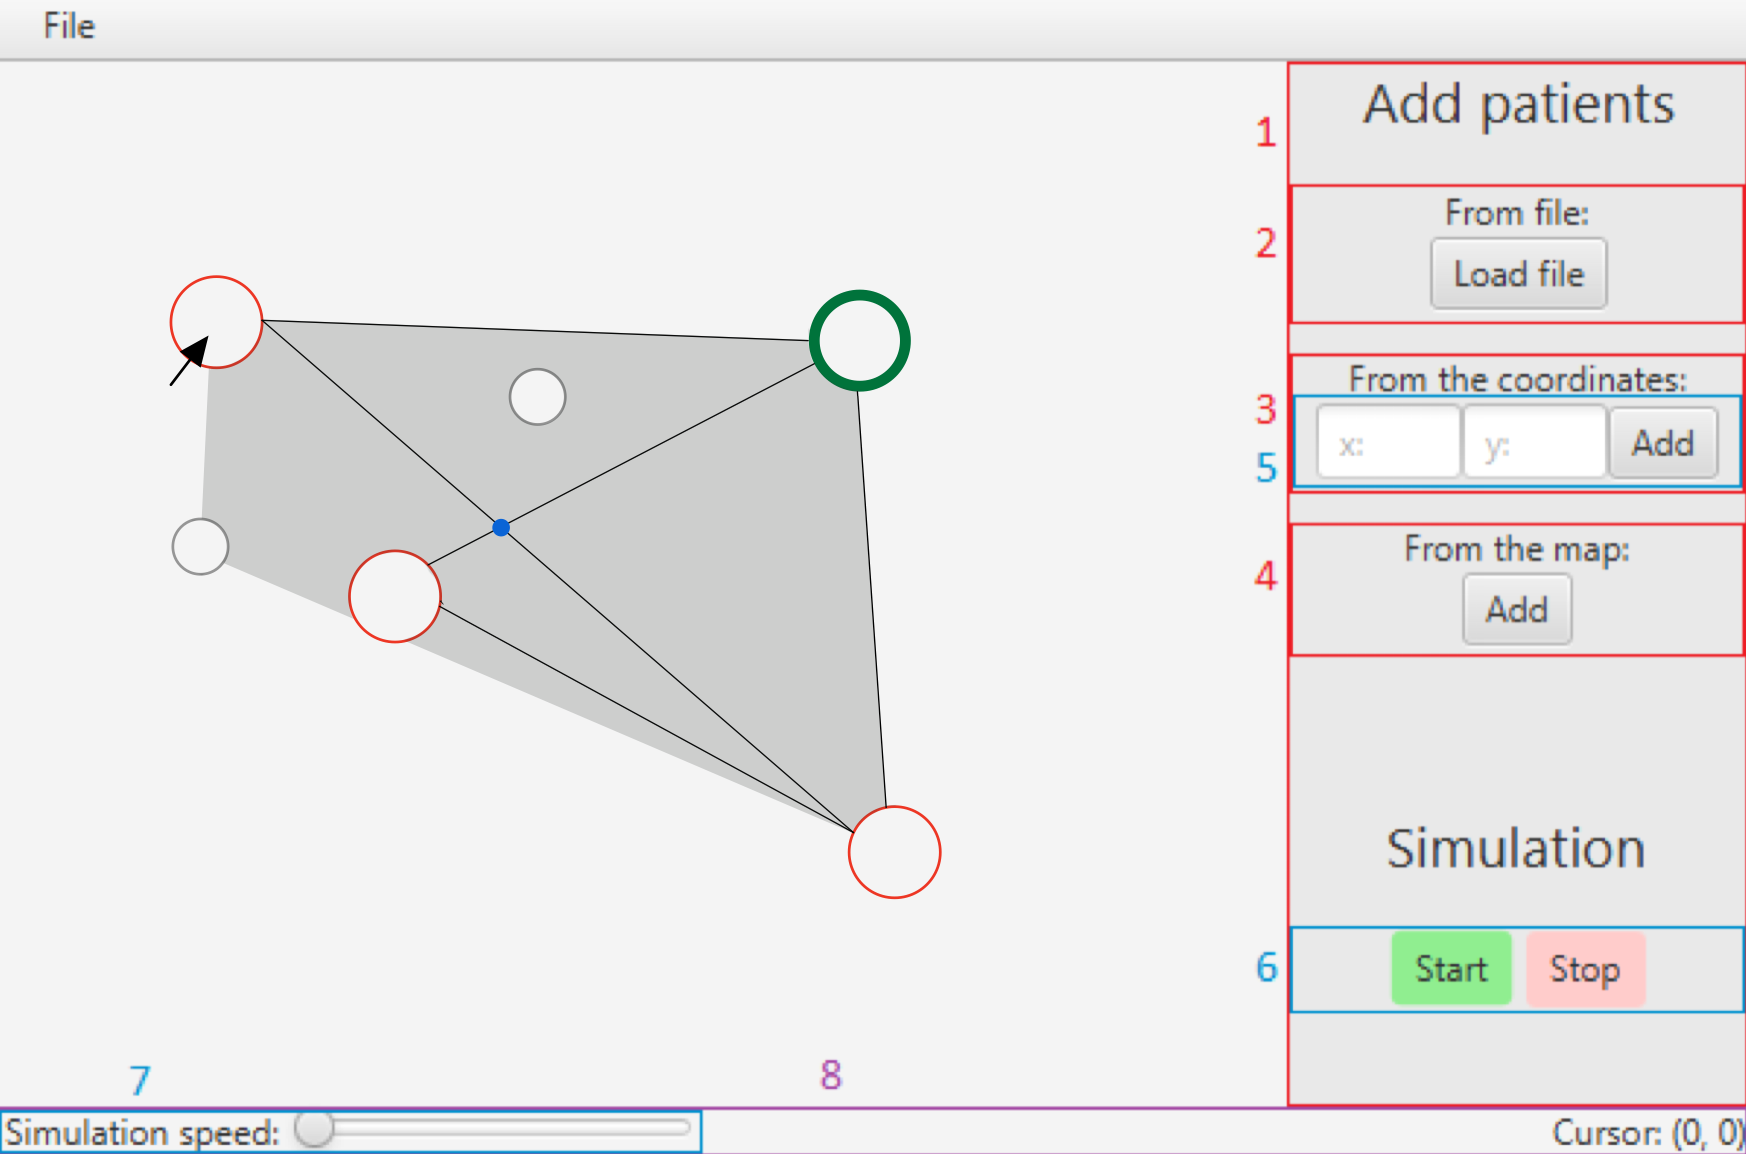
\includegraphics[width=\textwidth]{gui-impl.png}
                \caption{Ekran działania programu}
                \label{fig:GUI}
            \end{figure}
            
            Na zdjęciu zaznaczone są kontenery, kolorem:\\
                czerwonym - \textbf{VBox},\\
                niebieskim - \textbf{HBox},\\
                fioletowym - \textbf{BorderPane}.\\
            \\
            Głównym kontener w oknie jest \textbf{BorderPane}.\\
            Górna część - \textbf{MenuBar}(bez \textbf{MenuItem})\\
            Prawa część - \textbf{VBox}\\
            Dolna część - \textbf{BorderPane}\\
            Środkowa część - \textbf{Canvas}.\\
            \\
            W \textbf{VBox} 1 znajdziemy: \textbf{Label, VBox, VBox, VBox, Label, HBox}.\\
            W \textbf{VBox} 2: \textbf{Label, Button}.\\
            W \textbf{VBox} 3: \textbf{Label, HBox}.\\
            W \textbf{VBox} 4: \textbf{Label, Button}.\\
            W \textbf{HBox} 5: \textbf{TextField, TextField, Button}.\\
            W \textbf{HBox} 6: \textbf{Button, Button}.\\
            Lewą część \textbf{BorderPane} 8 wypełnia \textbf{HBox}, a prawą \textbf{Label}.
            W \textbf{HBox} 7 znajdziemy: \textbf{Label, Slider}.
            
        \subsection{Słuchacze akcji}
            W programie nasłuchiwane będą akcje z przycisków oraz z kursora myszy.
            Słuchacze następujących kontrolek, będą wywoływać następujące metody z klasy \textbf{Controller}:\\
            \begin{itemize}
                \item przycisk ,,File'' - loadMap()
                \item przycisk ,,Load file'' - loadPatientFromFile()
                \item przycisk ,,Add''(przy polach tekstowych x i y) - loadPatientFromCoordinates()
                \item przycisk ,,Add''(przy etykiecie ,,From the map:'') - loadPatientFromMap()
                \item przycisk ,,Start'' - startSimulation()
                \item przycisk ,,Stop'' - stopSimulation()
                \item ruch myszą - handleCursor()
            \end{itemize}
    
    \section{Testowanie}
        \subsection{Użyte narzędzia}
            Głównym narzędziem, za pomocą którego program zostanie przetestowany, będzie \textbf{JUnit 5}.
            Posłuży on nam do napisania testów jednostkowych metod w klasach.
            Dzięki temu, będziemy mogli przetestować pojedyncze funkcjonalności programu.\\
            Testy integralności tych funkcjonalności i testy graficznego interfejsu, zostaną przetestowane przez programistów ręcznie, w trakcie implementacji.
        
        \subsection{Konwencja}
            Testy danych klas za pomocą narzędzia \textbf{JUnit} zostaną napisane w odpowiadającej klasie i pakiecie
            w katalogu \textbf{test}.
            Metody testujące będą mieć nazwy odpowiadające temu, co metoda testuje.
            Użyta zostanie konwencja nazwnictwa metod testujących: \textbf{should + [co] + When + [warunek]}
            (np. shouldThrowIllegalArgumentExceptionWhenFilePathIsNull).\\
            Dzięki takiej konwencji rozmieszczenia plików testujących, łatwo znajdziemy testy danej klasy,
            a dzięki konwencji nazewnictwa metod, łatwo zrozumiemy co dana metoda testuje.
        
        \subsection{Warunki brzegowe}
            Wszystkie klasy z ważnymi i skomplikowanymi metodami, zostaną skrupulatnie przetestowane. Do tego zostaną użyte poprawne, jak i niepoprawne dane.
            \\
            Klasą, która jest najważniejsza jest klasa \textbf{PathFinder}. 
            Zostanie ona przetestowana dla danych zawierających różną liczbę połączeń pomiędzy szpitalami, a także gdy nie ma żądnych połączeń pomiędzy szpitalami.
            Testy będą się opierać głównie o to, by sprawdzić czy wyszukane połączenie, na pewno jest najkrótszym możliwym.
            Również zostanie wykonany test dla mapy, która nie zawiera żadnych szpitali.
            \\
            Klasy \textbf{MapFileReader} i \textbf{PatientsFileReader} są klasami najbardziej narażonymi na błędne dane.
            Zostaną one przetestowane, głównie dla danych niepoprawnych by sprawdzić
            czy algorytmy w nich zawarte potrafią znajdować błędy w pliku tekstowym.
            Te klasy zostaną przetestowane dla pustych plików oraz plików, które zawierają niepoprawne dane, takie jak:
            \begin{itemize}
                \item Liczby ujemne w miejscach gdzie są niedozwolone
                \item Powtarzające się id i nazwy (tylko w pliku z mapą)
                \item Połączenia pomiędzy nieistniejącymi szpitalami
                \item Dane, które nie są ani szpitalami, ani obiektami, ani drogami.
            \end{itemize}
            GUI zostanie przetestowane przez programistów ręcznie.
            Każda z kontrolek zostanie przetestowana pod względem poprawności działania.
            Sprawdzimy czy za pomocą suwaka szybkości animacji, można zatrzymać program.
            Sprawdzimy czy można uruchomić animację, gdy jest już ona uruchomiona.


\end{document}